\documentclass[]{spie}
%\documentclass[conference]{IEEEtran}
\usepackage[]{graphicx}
\usepackage{subfigure}
\usepackage{epsfig}

\usepackage[margin=0.5in,bottom=2in,top=1in]{geometry}
\usepackage{lastpage}
\usepackage{fancyhdr}
%\usepackage{algorithmic}
\usepackage[]{algorithm2e}
\usepackage{amsmath}
\usepackage{tabularx}

% =================
% =================

\setlength{\headheight}{45.9pt}
\pagestyle{fancy}
\lhead{}
\chead{}
\rhead{
		}
\lfoot{Scout based interior tomography
		}
\cfoot{
}
\rfoot{
Page \thepage
}
\renewcommand{\headrulewidth}{0pt}
\renewcommand{\footrulewidth}{0.4pt}



\usepackage{tikz}
\usetikzlibrary{shapes,arrows} 
\usepackage{hyperref}
\hypersetup{
    colorlinks,%
    citecolor=blue,%
    filecolor=blue,%
    linkcolor=blue,%
    urlcolor=blue
}


%\usepackage{setspace}
%\usepackage{amsmath}
%\usepackage{cite}
\let\useblackboard=\iftrue
%\topmargin -.5cm 
%\textheight 24cm \oddsidemargin -.75cm
%\textwidth 18.2cm
\useblackboard
\font\blackboard=msbm10 scaled \magstep1 \font\blackboards=msbm7
\font\blackboardss=msbm5
\newfam\black
\textfont\black=\blackboard \scriptfont\black=\blackboards
\scriptscriptfont\black=\blackboardss
\def\Bbb#1{{\fam\black\relax#1}}
\else
\def\Bbb{\bf}
\fi
\def\bra#1{\left\langle #1\right|}
\def\ket#1{\left| #1\right\rangle}
\newcommand{\ben}{\begin{eqnarray}\displaystyle}
\newcommand{\een}{\end{eqnarray}}
\newcommand{\et}{\emph{et al }}
\newcommand{\refb}[1]{(\ref{#1})}
%\newcommand{\sectiono}[1]{\section{#1}\setcounter{equation}{0}}
%\renewcommand{\theequation}{\thesection.\arabic{equation}}

\tikzstyle{decision} = [diamond, draw, fill=blue!20,  
    text width=8em, text badly centered, node distance=3cm, inner sep=0pt] 
\tikzstyle{block} = [rectangle, draw, fill=blue!20,  
    text width=8em, text centered, rounded corners, minimum height=4em, node distance=4cm] 
\tikzstyle{wideBlock} = [rectangle, draw, fill=blue!20,  
    text width=12em, text centered, rounded corners, minimum height=4em, node distance=4cm] 
\tikzstyle{autoBlock} = [rectangle, draw, fill=blue!20,  
   text centered, rounded corners, minimum height=4em, node distance=4cm] 
\tikzstyle{line} = [draw, -latex'] 
\tikzstyle{cloud} = [draw, ellipse,fill=red!20, 
    minimum height=4em, text width=8em, text centered, node distance=4.5cm] 
\tikzstyle{miniCloud} = [draw, ellipse,fill=red!20, 
    minimum height=4em, text width=5em, text centered, node distance=4.5cm] 
\tikzstyle{autoCloud} = [draw, ellipse,fill=red!20, 
    minimum height=4em, text centered, node distance=4.5cm] 
\tikzstyle{wideCloud} = [draw, ellipse,fill=red!20, 
    minimum height=4em, text width=14em, text centered, node distance=4.5cm] 
\tikzstyle{textBlock} = [ node distance=2cm, 
    minimum height=2em]     
\tikzstyle{imgBlock} = [rectangle, draw, fill=blue!20,  
     minimum height=4em, minimum width=4em] 

\begin{document}

\center{
{\LARGE \textbf{\textit{ScoutIT}:  \linebreak Interior Tomography using Modified Scout Acquisition}}
\linebreak
\vspace{1.5 cm} 
{\Large \textit{Kriti Sen Sharma} }
}
\tableofcontents
\setcounter{tocdepth}{0}

%\section{Abstract}


%%%%%%%%%%%%%%%%%%%%%%%%%%%%%%%%%%%%%%%%%%%%%%%%%%%%%%%%%%%%%%%%%%%%%%%%%
\section{Introduction}
\label{sec:introduction}

Xia et al. \cite{Xia2015} recently reported a method to improve image quality in truncated volume-of-interest (VOI) imaging using anterior-posterior (AP) and medio-lateral (ML) scout views. Their work was applied to C-arm based imaging, and relied on the assumption that the scout views cover the entire object, while the final VOI scan is severely truncated. In clinical computed tomography (CT), it is quite common that both the AP scout view and the final tomographic scan are moderately truncated, but the ML scout view is not truncated. This paper shows that acquiring AP scout views with a modified configuration allows accurate interior tomography for a truncated tomographic CT scan. 

%%%%%%%%%%%%%%%%%%%%%%%%%%%%%%%%%%%%%%%%%%%%%%%%%%%%%%%%%%%%%%%%%%%%%%%%%%
\section{Methods}
\label{sec:methods}

%+++++++++++++++++++++++++++++++++++++++++++++++++++++++++
%\subsection{Prior art}
%\label{ssec:prior_art}



%+++++++++++++++++++++++++++++++++++++++++++++++++++++++++
\subsection{Modified scout configuration}
\label{ssec:modified_scout}

Figure \ref{fig:blockdiag_mar2}A shows a normal scout configuration. The technologist typically attempts to align the patient at the iso-center (patient centering might not be accurate, and is typically improved through information gathered through the scouts). The source-to-(assumed)-iso-center distance is noted as $D_0$ in the figure. For  patients whose body-habitus does not lie within the FFOV of the scanner, the truncation predominantly arises in the AP direction but the lateral (ML) scouts are not truncated. 

\begin{figure}[hbtp]
\centering
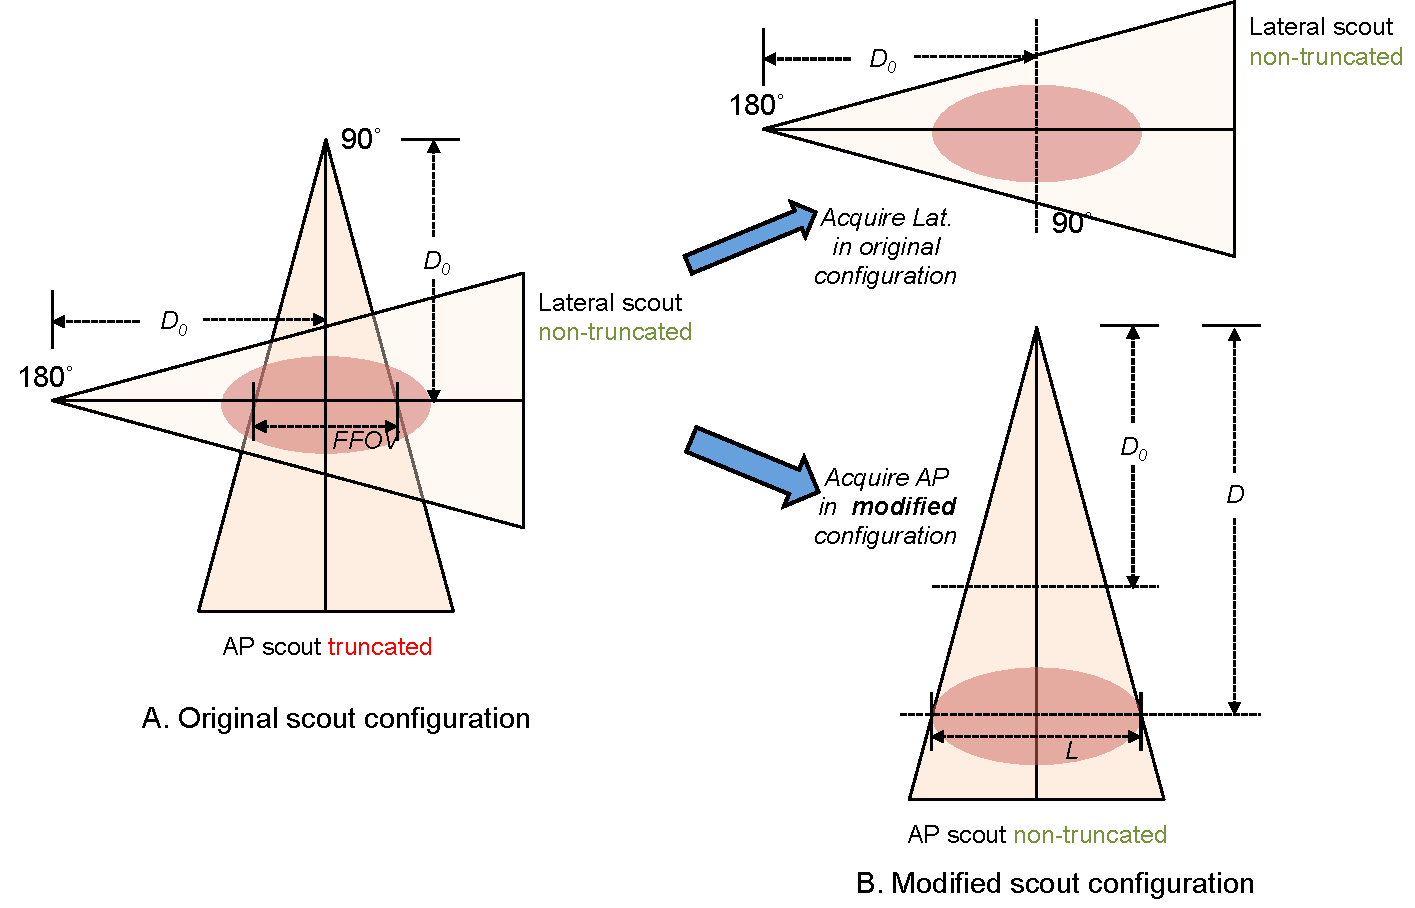
\includegraphics[width=15 cm]{figures/scoutIT_geometry}
\caption{Block diagram for two-pass metal artifact reduction algorithm (MAR2) \label{fig:blockdiag_mar2}
}
\end{figure}

As shown in Fig. \ref{fig:blockdiag_mar2}B, we propose a modified scout acquisition. While the lateral (ML) scouts are acquired in the original configuration, the AP scouts are acquired after moving the table down by a distance $d$ (there is of course a limit to how far the table can move down in the gantry). By moving the patient table down, the geometric magnification at the detector changes, and a larger patient habitus can be covered by x-ray beam. The modified AP scout configuration allows acquisition of non-truncated AP projections up to an extended body habitus of length $L_{eff}$, where:
\begin{align}
L = \frac{D}{D_0}\times FFOV
\end{align}

% TODO: Modify to generic CT system
We calculate the value for $L_{eff}$ for four CT scanners whose geometric specifications were reported in \cite{ImPACTCenterforEvidencebasedPurchasing2009}. We make the following assumptions:
\begin{itemize}
	\item the AP scouts are typically acquired at or near the actual iso-center
	\item the patient table can be moved down in the gantry by at least 150 mm; this appears to be a realistic estimate as the bore radius is greater than 400 mm for all the scanners in list below
\end{itemize}

Table \ref{tab:scanner_geoms} provides a list of relevant geometric specifications reproduced from  \cite{ImPACTCenterforEvidencebasedPurchasing2009}, the resulting value of $L_{eff}$ for a table displacement $d = 150 mm$, and the resulting percentage increase in patient habitus coverage. 

\begin{table}
\begin{center}
%\begin{tabular}{p{3 cm} p{3 cm} p{3 cm} p{3 cm} p{3 cm}}
%\begin{tabularx}{\linewidth}{l cccc}
\begin{tabular}{l cccc}
\hline 
\hline 
% & GE LightSpeed Xtra & Philips Brilliance Big Bore & Siemens SOMATOM Sensation Open (24 /40)  & Toshiba Aquilion LB  \\ 
 & GE LSX & Philips Br. & Siemens SOM.  & Toshiba Aq.  \\ 
\hline 
Aperture [cm]  & 80 & 85 & 82 & 90 \\ 
Focus-isocentre distance [mm]  & 606 & 645 & 570 & 712 \\ 
Focus-detector distance [mm]  & 1062.5 & 1183 & 1040 & 1275 \\ 
Maximum reconstruction field of view & 50 & 50 & 50 & 50 \\ 
Reconstruction matrices  & $512 \times 512$ & $512 \times 512$ & $512 \times 512$ & $512 \times 512$ \\ 
\hline 
$L_{eff}$ & 62.37 & 61.63 & 63.15 & 60.53 \\ 
\% increase & 24.75 & 23.26 & 26.32 & 21.07 \\ 
\hline 
\hline 
\end{tabular} 
\caption{Geometric specifications of four different CT scanners and corresponding values of increased patient coverage $L_{eff}$ \label{tab:scanner_geoms}}
\end{center}
\end{table}
%+++++++++++++++++++++++++++++++++++++++++++++++++++++++++
\subsection{Patient shape model estimation using slice-wise ellipse}
\label{ssec:ellipse-estimation}

%Xia et al. \cite{Xia2015} determined a best-fitting ellipse that described the boundaries in the non-truncated AP and lateral scout views. This ellipse is parameterized by the center $x_0$ and two radii $R_x$ and $R_y$. Their method uses only the boundary information from the scout views to determine this ellipse. As a simple explanation, the boundary from ML view is used to determine the radius of the ellipse along the \textit{y}-axis $R_y$. Figure \ref{fig:xia_ellipse} shows a figure from their paper showing the ellipse in relation to the AP and ML (lateral) scout views.

%\begin{figure}[hbtp]
%\centering
%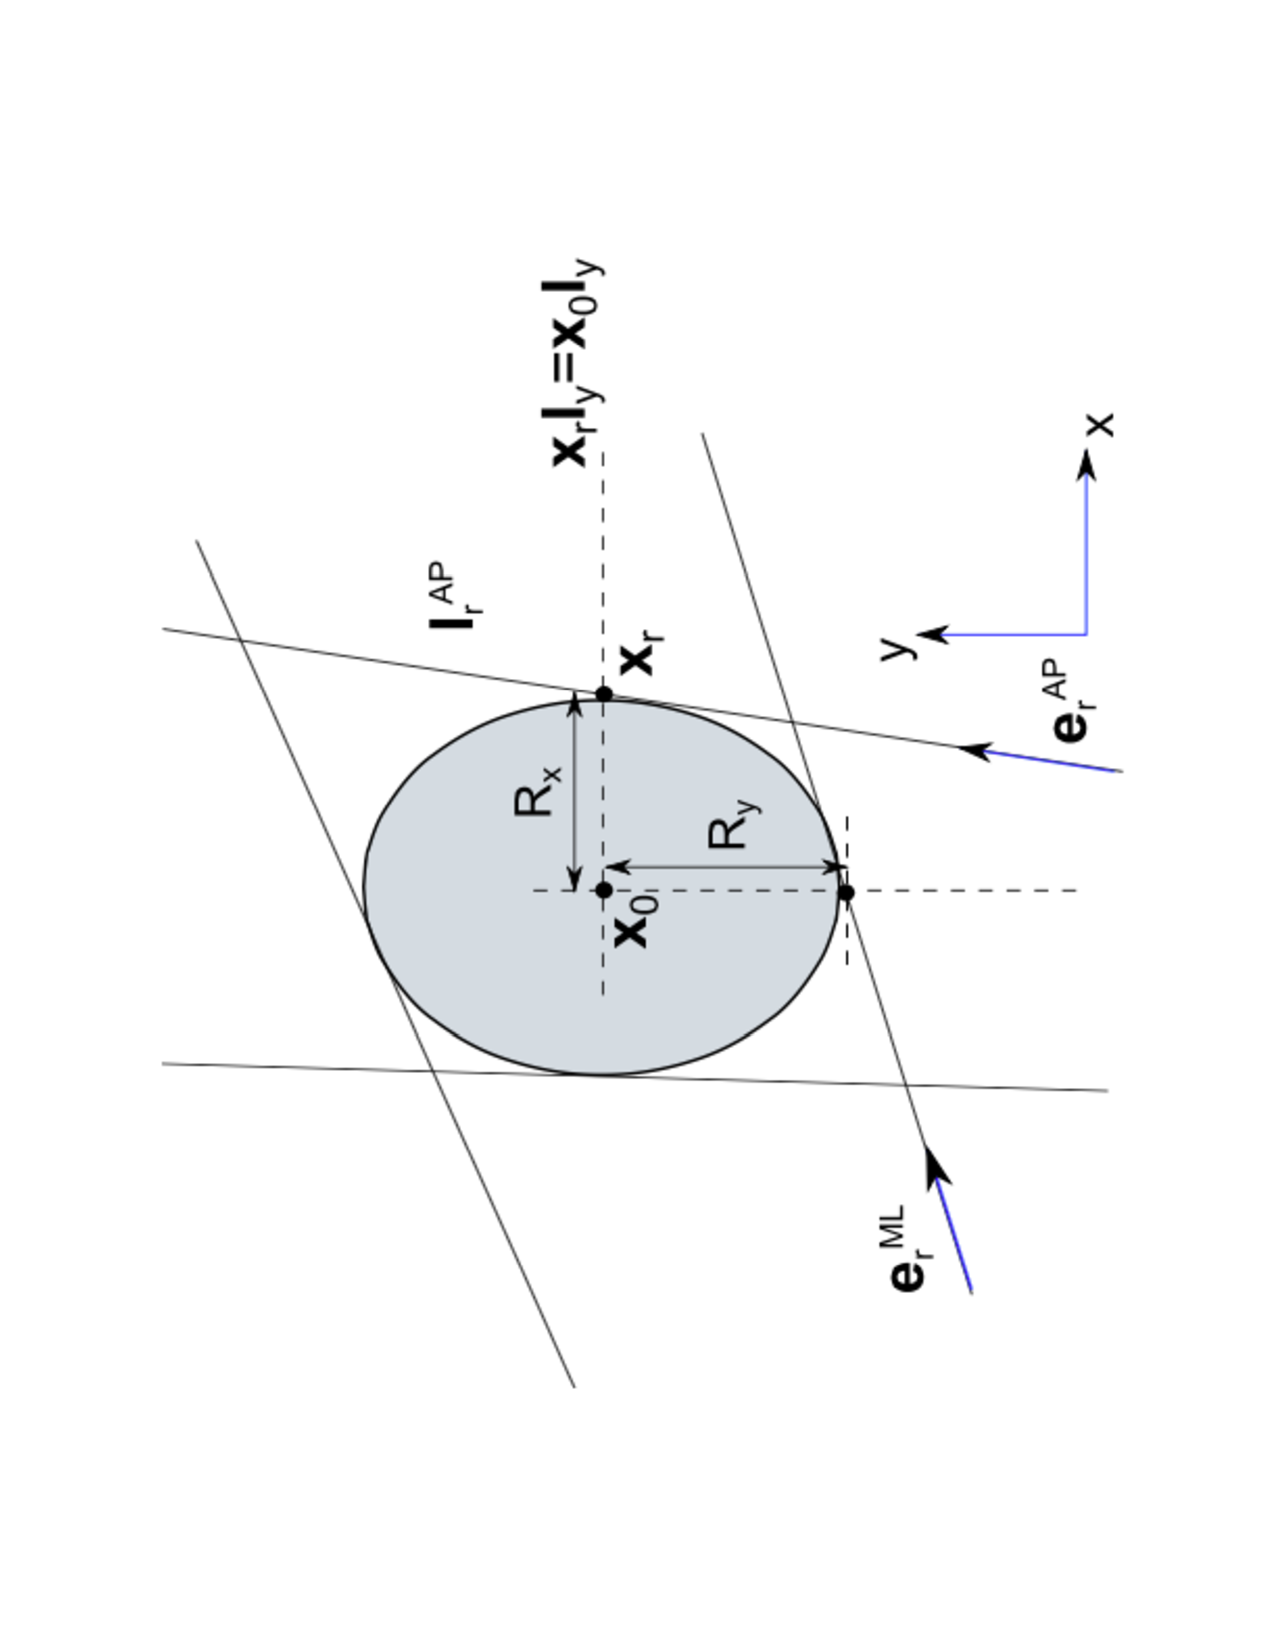
\includegraphics[width=15 cm]{figures/xia-ellipse-det}
%\caption{\textbf{From Xia et al. \cite{Xia2015}}: Illustration of how to approximate the ellipse radii $R_x$ and $R_y$ \label{fig:xia_ellipse}
%}
%\end{figure}
%
\begin{figure}[hbtp]
\centering
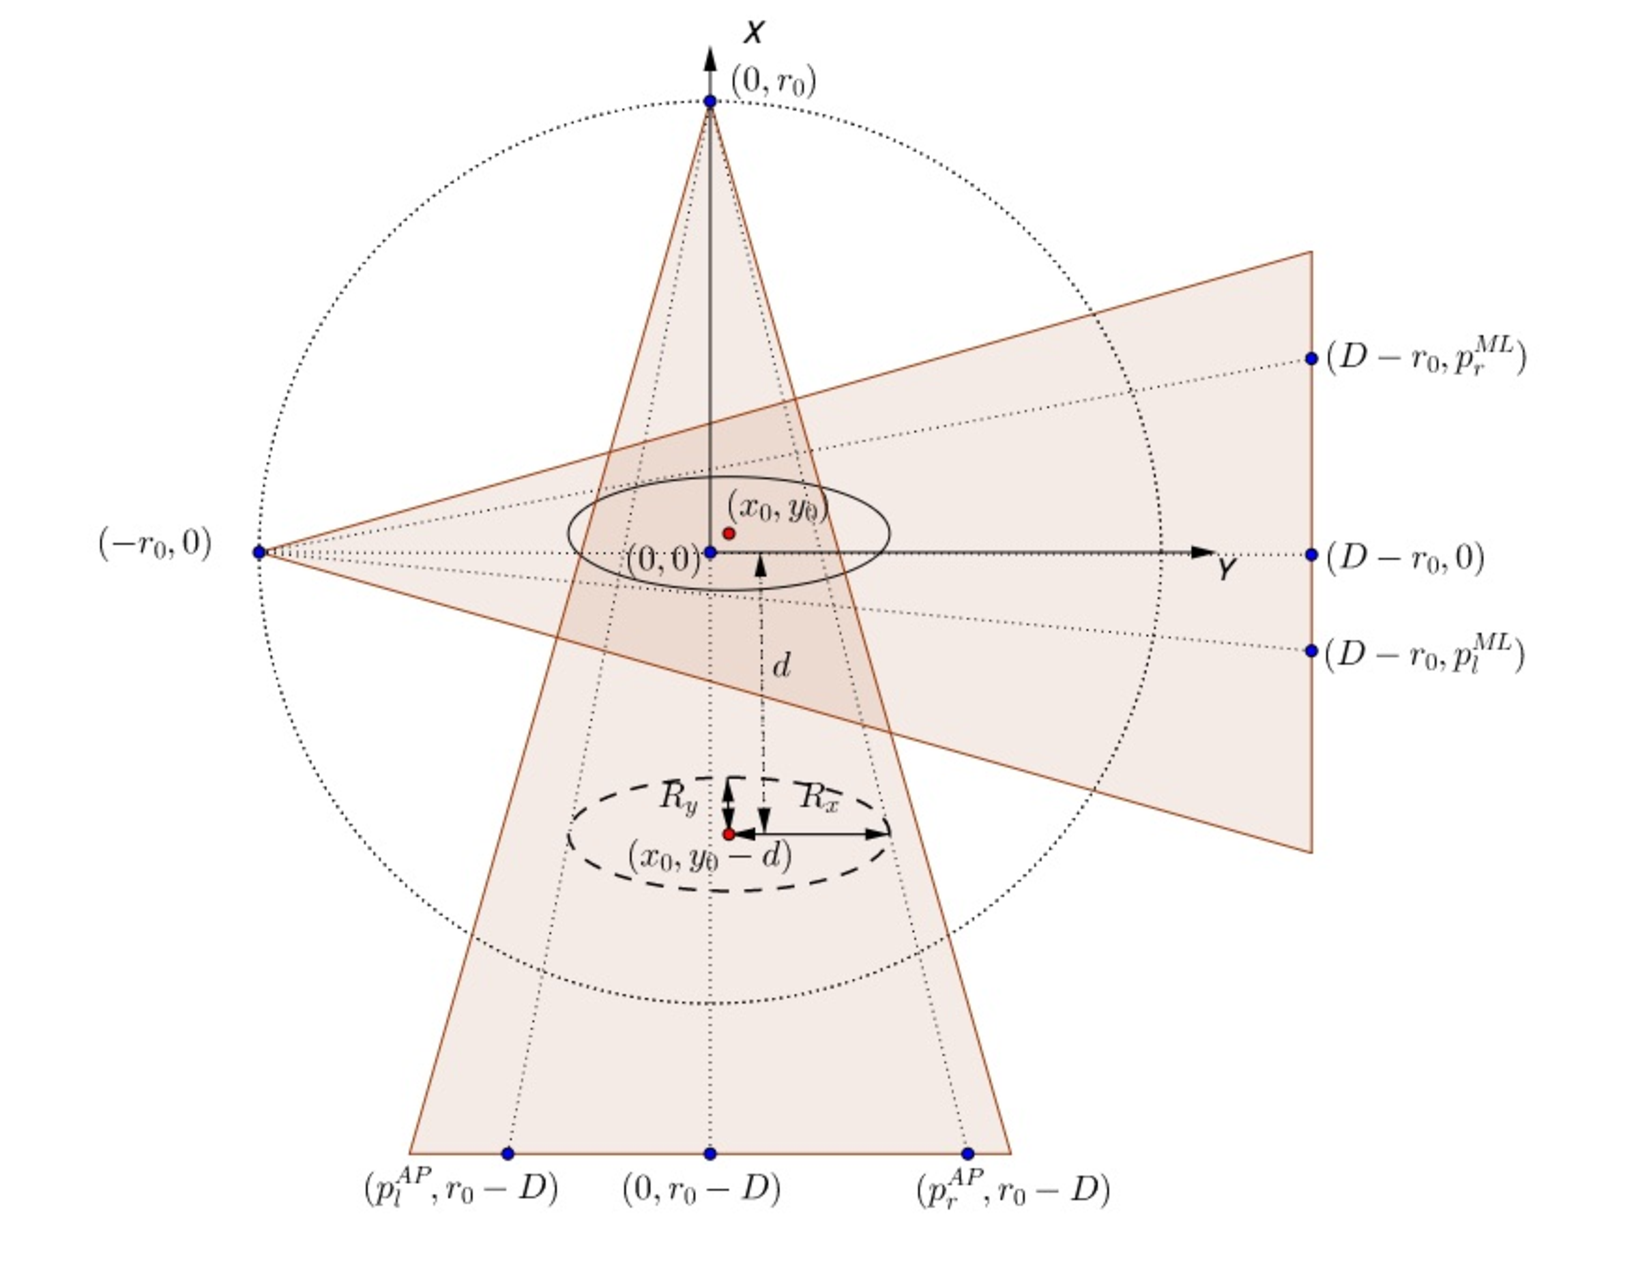
\includegraphics[width=15 cm]{figures/scoutIT_geometry-algebra}
\caption{Setup for acquisition of ML scout  in original configuration and AP scout in modified configuration \label{fig:scoutIT_geometry}
}
\end{figure}

In our setup shown in Fig. \ref{fig:scoutIT_geometry}, we place the origin of our co-ordinate axes $\left( 0, 0 \right)$ at the scanner iso-center. The source-to-iso-center distance is $r_0$ and the source-to-detector distance is $D$. Thus, the source is at $\left( 0, r_0 \right)$ when acquiring the AP view, and at $\left( -r_0, 0 \right)$ when acquiring the ML view. The patient's body habitus in the slice represented in this diagram is estimated as an ellipse with center $\left( x_0, y_0 \right)$ and major and minor axis lengths of $\left( R_X, R_y \right)$ respectively. 

As shown in the figure, the lateral (ML) scout is non-truncated in the original acquisition configuration. However, the AP scout would be truncated in this original configuration. By lowering the patient table by a distance $d$, the truncation is avoided. The projection of the iso-center, and tangents to the ellipse in the original ML scout and the modified AP scout are marked in the figure. In practice, these values are available from measurements on the acquired scout views. 

We calculate the slopes of the four tangents to the ellipse in ML and modified AP scout views as:
\begin{align}
m_l^{AP} &= \frac{-D}{p_l^{AP}} \nonumber \\
m_r^{AP} &= \frac{-D}{p_r^{AP}} \nonumber \\
m_l^{ML} &= \frac{p_l^{ML}}{D} \nonumber \\
m_r^{Ml} &= \frac{p_r^{ML}}{D} 
\end{align}
where the suffix $p_l$ and $p_r$ denote the left and right tangents. 

Next, we note the equation of the tangents below.

Tangents in ML scout:
\begin{equation}
\frac{y-0}{x-\left(-r_0 \right) } = m^{ML} \label{eqn:tangent_mlscout}
\end{equation}

Tangents in AP scout:
\begin{equation}
\frac{y-r_0}{x-0} = m^{AP} \label{eqn:tangent_apscout}
\end{equation}

The equation of the ellipse in the two configurations are noted below.

Ellipse in ML scout:
\begin{equation}
\left( \frac{y - y_0 }{R_y} \right)^2 + \left( \frac{x-x_0}{R_x}\right)^2 = 1 \label{eqn:ellipse_mlscout}
\end{equation}

Ellipse in modified AP scout configuration:
\begin{equation}
\left( \frac{y - \left( y_0 - d \right) }{R_y} \right)^2 + \left( \frac{x-x_0}{R_x}\right)^2 = 1 \label{eqn:ellipse_apscout}
\end{equation}

Now, the system of equations provided by equations  \ref{eqn:ellipse_mlscout} and \ref{eqn:tangent_mlscout} allow us to solve for the points of intersection of tangents to the ellipse in the ML scout. We apply the following operations on the system of equations:
\begin{enumerate}
	\item Though the value of $m_ML$ is known, we do not substitute this into the equation at first
	\item Substitute the equation for $y$ provided in Eq. \ref{eqn:tangent_mlscout} into Eq. \ref{eqn:ellipse_mlscout} \label{algo:subst1}
	\item Step \ref{algo:subst1} yields a quadratic in $x$. Since the the system of equation allows only a unique solution for each tangent, we can apply the formula that the discriminant of this quadratic is zero	 
\label{algo:discr}
	\item Step \ref{algo:discr} yields a quadratic in $m$. The parameters of the ellipse $\left\lbrace x_0, y_0, R_x, R_y \right\rbrace$ are also embedded in this equation
	\item Using the above quadratic which is of the form $A m^2 + B^m + C = 0$, we use the formulae for sum of roots and difference of roots
\end{enumerate}

By following the above set of steps for both the ML and AP scouts, we arrive at the following system of equations:
\begin{align}
\Sigma_1 \left( B x_0^2 - 1 \right) + 2 B x_0 \left( r_0 + d - y_0 \right) = 0  \nonumber \\
A \Delta_1^2 \left(B x^2 - 1 \right) - 4 B \left(A \left( r_0 + d - y_0 \right) ^2 + B x_0^2 - 1 \right) = 0 \nonumber \\
\Sigma_2 \left( B \left( x_0 + r_0 \right) ^2 - 1 \right) + 2 B y_0 \left( x_0 + r_0 \right) = 0  \nonumber  \\
A \Delta_2^2 \left(B \left( x_0 + r_0 \right) ^2 - 1 \right) - 4 B \left(A y_0^2 + B \left( x_0 + r_0 \right) ^2 - 1 \right) = 0 
\label{eq:finalsysofeqs}
\end{align}
where we used the following substitutions to simplify the equations:
\begin{align}
A = \frac{1}{R_y^2}  \nonumber  \\
B = \frac{1}{R_x^2}  \nonumber  \\
\Sigma_1 = m_l^{AP} + m_r^{AP} \nonumber  \\
\Sigma_2 = m_l^{ML} + m_r^{ML} \nonumber  \\
\Delta_1 = m_l^{AP} - m_r^{AP} \nonumber  \\
\Delta_2 = m_l^{ML} - m_r^{ML}
\end{align}

Thus we have a system of four equations with four unknowns $\left\lbrace x_0, y_0, R_x, R_y \right\rbrace$. This system can be solved with numerical solvers to yield the parameters of the ellipse (i.e. an estimate of the patient body habitus). 

%%%%%%%%%%%%%%%%%%%%%%%%%%%%%%%%%%%%%%%%%%%%%%%%%%%%%%%%%
\section{Results}
\label{sec:results}

Here we show experimental proof for the following:
\begin{itemize}
	\item \textbf{\textit{[Completed]}}: For Shepp-Logan phantom placed at an arbitrary displacement from iso-center, if ML scout is non-truncated and AP scout in modified configuration is non-truncated, then the four parameters of the ellipse are accurately determined. Example below:
		\begin{itemize}
			\item Shepp Logan phantom was expressed into a $512 \times 512$ image grid. The major and minor axes were measured manually as $R_x $ and $R_y $ pixels. A perturbation from iso-center $(x_0, y_0)$ was introduced. Thus we ran simulations using $\left\lbrace x_0 = -5, y_0 = -8, R_x = 233 , R_y = 177 \right\rbrace$
			\item Scout projections were generated using OpenRecon forward projector codes
			\item The AP scout was truncated (and ML scout was non-truncated) in the original configuration. By moving the detector down by 200 mm, a non-truncated AP scout was acquired. 
			\item The edges of the non-truncated scout views were measured and the slope of the tangents were calculated using equations \ref{eqn:tangent_mlscout} and \ref{eqn:tangent_apscout}
			\item Finally, the system of equations \ref{eq:finalsysofeqs} was solved to determine the unknowns $\left\lbrace x_0 = -4.89, y_0 = -8.16, R_x = 233 , R_y = 173 \right\rbrace$
			\item We noted that the calculated values matched the simulation parameters closely
		\end{itemize}
	\item \textbf{\textit{[Completed, need to add description]}}: Next, we showed that knowledge of the patient habitus (approximated by an ellipse) led to more accurate interior tomography than existing methods (that do not use knowledge acquired from the scout views)
	\item \textbf{\textit{[To be done]}}: Finally, we show the same trend in results for real clinical data for obese patient cases
\end{itemize}

%=========================================================================


%%%%%%%%%%%%%%%%%%%%%%%%%%%%%%%%%%%%%%%%%%%%%%%%%%%%%%%%%%%%%%%%%%%%%%%%%%

%%%%%%%%%%%%%%%%%%%%%%%%%%%%%%%%%%%%%%%%%%%%%%%%%%%%%%%%%%%%%%%%%%%%%%%%%%
\bibliography{bibl_scoutit}   %>>>> bibliography data in prelim.bib
\bibliographystyle{spiebib}   %>>>> makes bibtex use spiebib.bst


\end{document}
